\documentclass[12pt,letterpaper]{article}

% ---- Packages ----
\usepackage[utf8]{inputenc}
\usepackage{graphicx}
\usepackage{natbib}
\usepackage{setspace}
\usepackage{fullpage}
\usepackage{amsmath,amssymb}
\usepackage{hyperref}
\usepackage{xcolor}
\usepackage[compact]{titlesec}
\usepackage{booktabs}
\usepackage{siunitx}
\usepackage{tabularray}
\UseTblrLibrary{siunitx}
\usepackage{listings}
\usepackage{caption}
\usepackage{placeins}

% ---- Formatting ----
\setlength{\parindent}{0pt}
\setlength{\parskip}{0.75em}
\onehalfspacing

\hypersetup{
	colorlinks=true,
	linkcolor=blue,
	citecolor=blue,
	urlcolor=blue
}

\captionsetup{font=small}

\lstset{
	language=R,
	basicstyle=\ttfamily\small,
	breaklines=true,
	frame=single,
	numbers=left,
	numberstyle=\tiny,
	stepnumber=1,
	numbersep=8pt,
	showstringspaces=false,
	tabsize=2,
	xleftmargin=1.5em,
	framexleftmargin=1.2em
}

% ---- Title ----
\title{Replication Report: Democratic Sanctions and the Selective Targeting of Authoritarian Regimes}
\date{Applied Statistical Analysis II \\ Trinity College Dublin \\ \today}
\author{Jakob L\"utkemeier}

\begin{document}
	\maketitle
	
	% Assumes this .tex file lives inside the reports/ folder, with
	% tables/ and figures/ as subfolders. If your file lives elsewhere,
	% adjust the relative paths in \input{} and \includegraphics{}.
	
	\section*{Abstract}
	
	This report replicates the core empirical findings of Christian von Soest and Michael Wahman's study of democratic sanctions against authoritarian regimes and adds one modest extension. The original article argues that Western democratic sanctions are shaped not only by authoritarian repression itself, but by a selective cost--benefit calculus involving trigger events, target vulnerability, and sender costs. Using the provided replication data, I reproduced the paper's main outputs for the trigger models, the post-estimation probability changes, the selective-targeting models, and the FDI interaction figure. Substantively, the replication was successful: the central findings on coups, controversial elections, selective targeting, and the role of foreign direct investment were recovered closely enough to support the paper's main claims. I then extend the analysis by testing whether controversial elections are less likely to trigger sanctions when targets are especially politically aligned with the West, operationalized as the top quartile of UN voting similarity. The extension is suggestive rather than decisive. The interaction points in the expected negative direction, but uncertainty remains substantial and descriptive support is more convincing than formal inferential strength.
	
	\section{Introduction}
		
	The original article by  \citet{vonsoestNotAllDictators2015}, ``Not all dictators are equal: Coups, fraudulent elections, and the selective targeting of democratic sanctions," studies democratic sanctions imposed by the United States and the European Union against authoritarian regimes after the Cold War. The motivating puzzle is straightforward: some authoritarian regimes with extremely poor democratic and human-rights records are never sanctioned, while others face repeated sanction episodes. Von Soest and Wahman argue that sanctions are therefore not a simple reflection of how repressive a regime is. Instead, sanctioning is selective. Western senders respond especially strongly to dramatic trigger events, but they also weigh the vulnerability of the target and their own expected political and economic costs before acting \citep{vonsoestNotAllDictators2015}.
	
	The report proceeds as follows. Section 2 summarizes the original study's argument and hypotheses. Section 3 describes the data, modelling strategy, and scope of the replication. Section 4 presents the main replication results. Section 5 introduces and evaluates my extension, a controversial election $\times$ high political closeness interaction. Section 6 concludes by assessing how well the replication worked and what the extension does, and does not, add.
	
	\section{The Original Study}
	
	%\subsection*{Research question and theoretical logic}
	
	Von Soest and Wahman ask: under what conditions do the main Western sanction senders, the United States and the European Union, impose democratic sanctions on authoritarian regimes? Their key contribution is to treat sanction onset as a selective political decision rather than as an automatic reaction to repression. Democratic sanctions, in their definition, are sanctions that explicitly seek improvements in democracy or human rights rather than unrelated objectives such as anti-terrorism or anti-proliferation \citep{vonsoestNotAllDictators2015}.
	
	The paper organizes the sanction decision around three components of a sender-side cost--benefit calculus. First, there is \emph{pressure to sanction}. Dramatic trigger events such as coups d'\'etat and internationally controversial elections attract public and diplomatic attention and therefore heighten pressure on Western governments to act. Second, there is \emph{target vulnerability}. Senders should be more willing to sanction regimes that appear politically or economically vulnerable, because the probability of influencing their behaviour is greater. Third, there are \emph{sender costs}. Even when democratic norms are violated, Western governments may hesitate if the target is politically aligned with them or economically important to them \citep{vonsoestNotAllDictators2015}.
	
	This logic leads to a clean set of empirical expectations. The first hypothesis is that dramatic trigger events, especially coups, should be powerful predictors of democratic sanctions. The second is that vulnerable regimes should be more likely to be sanctioned. The third is that sanctions should be less likely when the expected political and economic costs to the sender are high. A particularly important nuance in the paper is that ``weaker'' triggers such as controversial elections leave more room for strategic discretion than coups. That is why the original article interacts controversial elections with foreign direct investment (FDI): if a trigger is less overwhelming, costly targets may be protected more easily \citep{vonsoestNotAllDictators2015}.

	\subsection*{Data and empirical strategy}
	
	The study uses a newly compiled dataset of democratic sanctions issued by the United States and the European Union against authoritarian regimes in the post-Cold War period, covering 1990--2010 \citep{vonsoestNotAllDictators2015}. The dependent variable is democratic sanction onset: in the main specification, the authors merge EU and US democratic sanctions and code the first year in which either sender imposes such a sanction as the onset year; they also estimate supplementary models for EU and US sanctions separately. Country-years in which a democratic sanction was already in place at $t-1$ are excluded, because those cases do not represent a new sanctioning decision.
	
	The authors estimate a series of logistic regression models because the outcome of interest is binary: whether a democratic sanction begins in a given country-year. Standard errors are clustered by country to account for within-country dependence across repeated observations over time. To address temporal dependence in sanction onset, the models also include cubic polynomials of time since the last sanction event, following standard practice for binary time-series cross-sectional data. Most independent variables are lagged by one year, while the trigger variables and protests are not lagged because sanctions are expected to follow those events promptly \citep{vonsoestNotAllDictators2015}.
	
	A further detail worth clarifying is the distinction between HTW and BMR in the tables. HTW refers to the Hadenius \& Teorell authoritarian-sample definition, updated by Wahman, Teorell, and Hadenius, which is the paper's main sample because it aligns with the authors' continuous understanding of democracy. BMR refers to the alternative authoritarian classification by Boix, Miller, and Rosato. The paper includes BMR models as a robustness check to show that the main findings are not an artefact of one particular regime-classification rule. In Table I, for example, Model 1 is the main HTW specification, Model 2 repeats the analysis on the BMR sample, and Models 3 and 4 then separate EU and US sanctions within the HTW setup.
	
	The replication script follows this design closely. It reconstructs the lagged dependent variables needed for the sanction-onset sample restrictions, builds model-specific samples through listwise deletion and exclusion of country-years already under democratic sanction at $t-1$, and then estimates the paper's core logit models. For this report, I keep the focus on the paper's main outputs: Table I, Table II, Table III, and the article's Figure 2.	
	
	\section{Main Replication Results}
	
	The original study did not provide an R workflow. Instead, the replication materials consisted of a Stata \texttt{.do} file and \texttt{.dta} dataset, so I first translated that setup into R. Specifically, \texttt{parse\_stata.R} reads the original Stata data with \texttt{haven}, inspects variable structure and labels, exports a CSV version, and prints the \texttt{.do} file so the original model sequence is transparent; on that basis, \texttt{replication\_analysis.R} reconstructs only the missing lagged dependent variables needed for sample restrictions, translates the clustered logit models and main post-estimation steps into R, and saves the resulting tables and figures for the report.	
	
	\subsection*{Triggers for democratic sanctions}
	
	The first replication block concerns the paper's trigger argument. The authors claim that democratic sanctions respond much more strongly to dramatic trigger events than to static or slowly moving measures of authoritarianism. In practical terms, this means that coups and controversial elections should matter more than low democracy levels per se or gradual deterioration in civil liberties.
	
	\begin{table}
	\centering
	\begin{talltblr}[         %% tabularray outer open
		caption={Triggers of democratic sanctions},
		]                     %% tabularray outer close
		{                     %% tabularray inner open
			colspec={Q[]Q[]Q[]Q[]Q[]},
			hline{2}={1-5}{solid, black, 0.05em},
			hline{36}={1-5}{solid, black, 0.05em},
			hline{1}={1-5}{solid, black, 0.08em},
			hline{37}={1-5}{solid, black, 0.08em},
			column{2-5}={}{halign=c},
			column{1}={}{halign=l},
		}                     %% tabularray inner close
		& \shortstack{(1) HTW\\(Western)} & \shortstack{(2) BMR\\(Western)} & \shortstack{(3) HTW\\(EU)} & \shortstack{(4) HTW\\(US)} \\
		Coup & \num{5.127}*** & \num{4.869}*** & \num{3.765}*** & \num{4.947}*** \\
		& (\num{0.765}) & (\num{0.645}) & (\num{0.697}) & (\num{0.681}) \\
		Democracy score (0--10) & \num{-0.056} & \num{-0.040} & \num{-0.081} & \num{-0.116} \\
		& (\num{0.089}) & (\num{0.095}) & (\num{0.090}) & (\num{0.111}) \\
		Controversial election & \num{2.584}*** & \num{2.434}*** & \num{2.620}*** & \num{2.275}*** \\
		& (\num{0.459}) & (\num{0.408}) & (\num{0.466}) & (\num{0.496}) \\
		Change in civil liberties & \num{0.411} & \num{0.453} & \num{0.368} & \num{0.349} \\
		& (\num{0.319}) & (\num{0.355}) & (\num{0.364}) & (\num{0.418}) \\
		Non-democratic sanction ($t-1$) & \num{0.053} & \num{0.031} & \num{-0.273} & \num{-0.523} \\
		& (\num{0.624}) & (\num{0.656}) & (\num{0.783}) & (\num{1.002}) \\
		Time since last sanction & \num{-1.788}** &  &  &  \\
		& (\num{0.553}) &  &  &  \\
		Time since last sanction$^2$ & \num{0.226}** &  &  &  \\
		& (\num{0.083}) &  &  &  \\
		Time since last sanction$^3$ & \num{-0.008}* &  &  &  \\
		& (\num{0.003}) &  &  &  \\
		Time since last sanction (BMR) &  & \num{-1.159}* &  &  \\
		&  & (\num{0.501}) &  &  \\
		Time since last sanction$^2$ (BMR) &  & \num{0.140}* &  &  \\
		&  & (\num{0.068}) &  &  \\
		Time since last sanction$^3$ (BMR) &  & \num{-0.005}+ &  &  \\
		&  & (\num{0.003}) &  &  \\
		Time since last EU sanction &  &  & \num{-1.439}* &  \\
		&  &  & (\num{0.599}) &  \\
		Time since last EU sanction$^2$ &  &  & \num{0.191}* &  \\
		&  &  & (\num{0.095}) &  \\
		Time since last EU sanction$^3$ &  &  & \num{-0.007}+ &  \\
		&  &  & (\num{0.004}) &  \\
		Time since last US sanction &  &  &  & \num{-2.067}** \\
		&  &  &  & (\num{0.650}) \\
		Time since last US sanction$^2$ &  &  &  & \num{0.253}** \\
		&  &  &  & (\num{0.093}) \\
		Time since last US sanction$^3$ &  &  &  & \num{-0.009}* \\
		&  &  &  & (\num{0.004}) \\
		N & \num{1520} & \num{1529} & \num{1668} & \num{1583} \\
	\end{talltblr}
\end{table}

	The replicated Table I supports that interpretation well. Across the main Western-sanctions specification and the EU- and US-specific variants, coups emerge as the strongest and most consistent predictor of sanction onset. Controversial elections are also positively associated with sanctions and remain substantively important. By contrast, the level of democracy and the change in civil liberties are much weaker in the core models. This is the first major respect in which the replication was successful: it reproduces the paper's central claim that Western democratic sanctions are most clearly triggered by dramatic and visible events rather than by persistently low democratic quality alone.
	
	\begin{table}
\centering
\begin{talltblr}[         %% tabularray outer open
caption={Change in predicted probability of democratic sanctions},
]                     %% tabularray outer close
{                     %% tabularray inner open
colspec={Q[]Q[]Q[]Q[]},
hline{2}={1-4}{solid, black, 0.05em},
hline{1}={1-4}{solid, black, 0.08em},
hline{8}={1-4}{solid, black, 0.08em},
column{1-4}={}{halign=l},
}                     %% tabularray inner close
Statistic & Western sanction & EU sanction & US sanction \\
\shortstack[l]{Baseline probability\\(no coup, no controversial election)} & 0.007 & 0.007 & 0.004 \\
90\% Conf. interval & 0.003–0.014 & 0.003–0.017 & 0.002–0.008 \\
Coup & 0.519 & 0.232 & 0.346 \\
90\% Conf. interval & 0.274–0.764 & 0.052–0.412 & 0.074–0.618 \\
Internationally controversial election & 0.074 & 0.084 & 0.032 \\
90\% Conf. interval & 0.010–0.137 & 0.004–0.163 & 0.004–0.060 \\
\end{talltblr}
\end{table}

	
	The replicated Table II reinforces the same story in a more interpretable form. Baseline sanction probabilities remain low when no major trigger is present, but coups generate a very large increase in the probability of sanction onset, while controversial elections generate a smaller yet still meaningful increase. That ordering is exactly what the theory predicts: coups provide the clearest mandate for coercive foreign-policy action, whereas controversial elections are weaker triggers that still matter but leave more discretion to the sender.
	
	\FloatBarrier
	
	\subsection*{Selective targeting and sender costs}
	
	The next replication step tests the broader theory of selective targeting. If democratic sanctions are selective, then they should depend not only on trigger events but also on target vulnerability and sender costs.
	
	\begin{table}
	\centering
	\begin{talltblr}[         %% tabularray outer open
		caption={Determinants of democratic sanctions},
		]                     %% tabularray outer close
		{                     %% tabularray inner open
			colspec={Q[]Q[]Q[]Q[]},
			rowsep=1pt,
			hline{2}={1-4}{solid, black, 0.05em},
			hline{42}={1-4}{solid, black, 0.05em},
			hline{1}={1-4}{solid, black, 0.08em},
			hline{43}={1-4}{solid, black, 0.08em},
			column{2-4}={}{halign=c},
			column{1}={}{halign=l},
		}                     %% tabularray inner close
		& \shortstack{(5) HTW\\(Western)} & \shortstack{(6) BMR\\(Western)} & \shortstack{(7) HTW\\(Western)} \\
		Coup & \num{5.128}*** & \num{5.050}*** & \num{5.121}*** \\
		& (\num{1.001}) & (\num{0.817}) & (\num{1.021}) \\
		Controversial election & \num{2.909}*** & \num{2.881}*** & \num{3.278}*** \\
		& (\num{0.452}) & (\num{0.415}) & (\num{0.499}) \\
		Protests & \num{0.095} & \num{0.123}+ & \num{0.090} \\
		& (\num{0.060}) & (\num{0.063}) & (\num{0.066}) \\
		GDP per capita growth ($t-1$) & \num{-0.026} & \num{-0.024} & \num{-0.023} \\
		& (\num{0.030}) & (\num{0.035}) & (\num{0.030}) \\
		Inflation ($t-1$) & \num{0.022}** & \num{0.031}*** & \num{0.022}** \\
		& (\num{0.008}) & (\num{0.009}) & (\num{0.008}) \\
		GDP per capita (\$1,000s, $t-1$) & \num{-0.178}* & \num{-0.115} & \num{-0.181}* \\
		& (\num{0.089}) & (\num{0.091}) & (\num{0.089}) \\
		Western organizational ties ($t-1$) & \num{0.301}* & \num{0.338}* & \num{0.316}** \\
		& (\num{0.117}) & (\num{0.133}) & (\num{0.115}) \\
		China/Russia ties ($t-1$) & \num{-0.081} & \num{-0.107} & \num{-0.048} \\
		& (\num{0.157}) & (\num{0.161}) & (\num{0.162}) \\
		Western trade, log ($t-1$) & \num{-0.083} & \num{-0.073} & \num{-0.091} \\
		& (\num{0.174}) & (\num{0.135}) & (\num{0.176}) \\
		FDI inflows ($t-1$) & \num{-0.046}* & \num{-0.057}*** & \num{-0.029} \\
		& (\num{0.022}) & (\num{0.016}) & (\num{0.036}) \\
		Oil production ($t-1$) & \num{0.001} & \num{-0.001} & \num{0.002} \\
		& (\num{0.007}) & (\num{0.008}) & (\num{0.007}) \\
		Non-democratic sanction ($t-1$) & \num{0.848} & \num{0.483} & \num{0.870} \\
		& (\num{0.571}) & (\num{0.709}) & (\num{0.564}) \\
		Political closeness to West ($t-1$) & \num{-4.413}** & \num{-5.587}** & \num{-4.495}* \\
		& (\num{1.651}) & (\num{1.844}) & (\num{1.753}) \\
		Time since last sanction & \num{-1.643}** &  & \num{-1.706}** \\
		& (\num{0.572}) &  & (\num{0.603}) \\
		Time since last sanction$^2$ & \num{0.212}* &  & \num{0.224}* \\
		& (\num{0.083}) &  & (\num{0.089}) \\
		Time since last sanction$^3$ & \num{-0.008}* &  & \num{-0.009}* \\
		& (\num{0.003}) &  & (\num{0.004}) \\
		Time since last sanction (BMR) &  & \num{-0.758} &  \\
		&  & (\num{0.498}) &  \\
		Time since last sanction$^2$ (BMR) &  & \num{0.098} &  \\
		&  & (\num{0.065}) &  \\
		Time since last sanction$^3$ (BMR) &  & \num{-0.004} &  \\
		&  & (\num{0.002}) &  \\
		Controversial election $\times$ FDI inflows &  &  & \num{-0.236}+ \\
		&  &  & (\num{0.121}) \\
		N & \num{1219} & \num{1229} & \num{1219} \\
	\end{talltblr}
\end{table}
	
	The replicated Table III recovers the main structure of the original results convincingly. First, the trigger variables remain important even after adding the broader set of controls, which indicates that the trigger story was not an artefact of omitted structural variables. Second, the signs and substantive interpretation of the vulnerability and sender-cost variables are broadly consistent with the article. In particular, politically closer regimes are less likely to be sanctioned, and higher FDI is associated with lower sanction propensity. At the same time, the positive and significant inflation coefficient points to the vulnerability side of the argument: economically unstable regimes appear more likely to be sanctioned, which fits the paper’s expectation that senders are more willing to target countries that look politically or economically fragile. This is exactly the selective-targeting logic of the paper: even when democratic norms are violated, Western senders are less inclined to sanction countries from which they expect higher political or economic costs, but more inclined to act where target vulnerability suggests a greater chance of pressure succeeding.
	
	Model 7 then adds the article's central interaction between controversial elections and FDI. The theoretical motivation is that controversial elections are weaker triggers than coups and therefore provide more room for selective enforcement. If so, the constraining role of sender costs should be especially visible after controversial elections. The margins plot below reproduces that argument graphically.
	
	\begin{figure}[htbp]
		\centering
		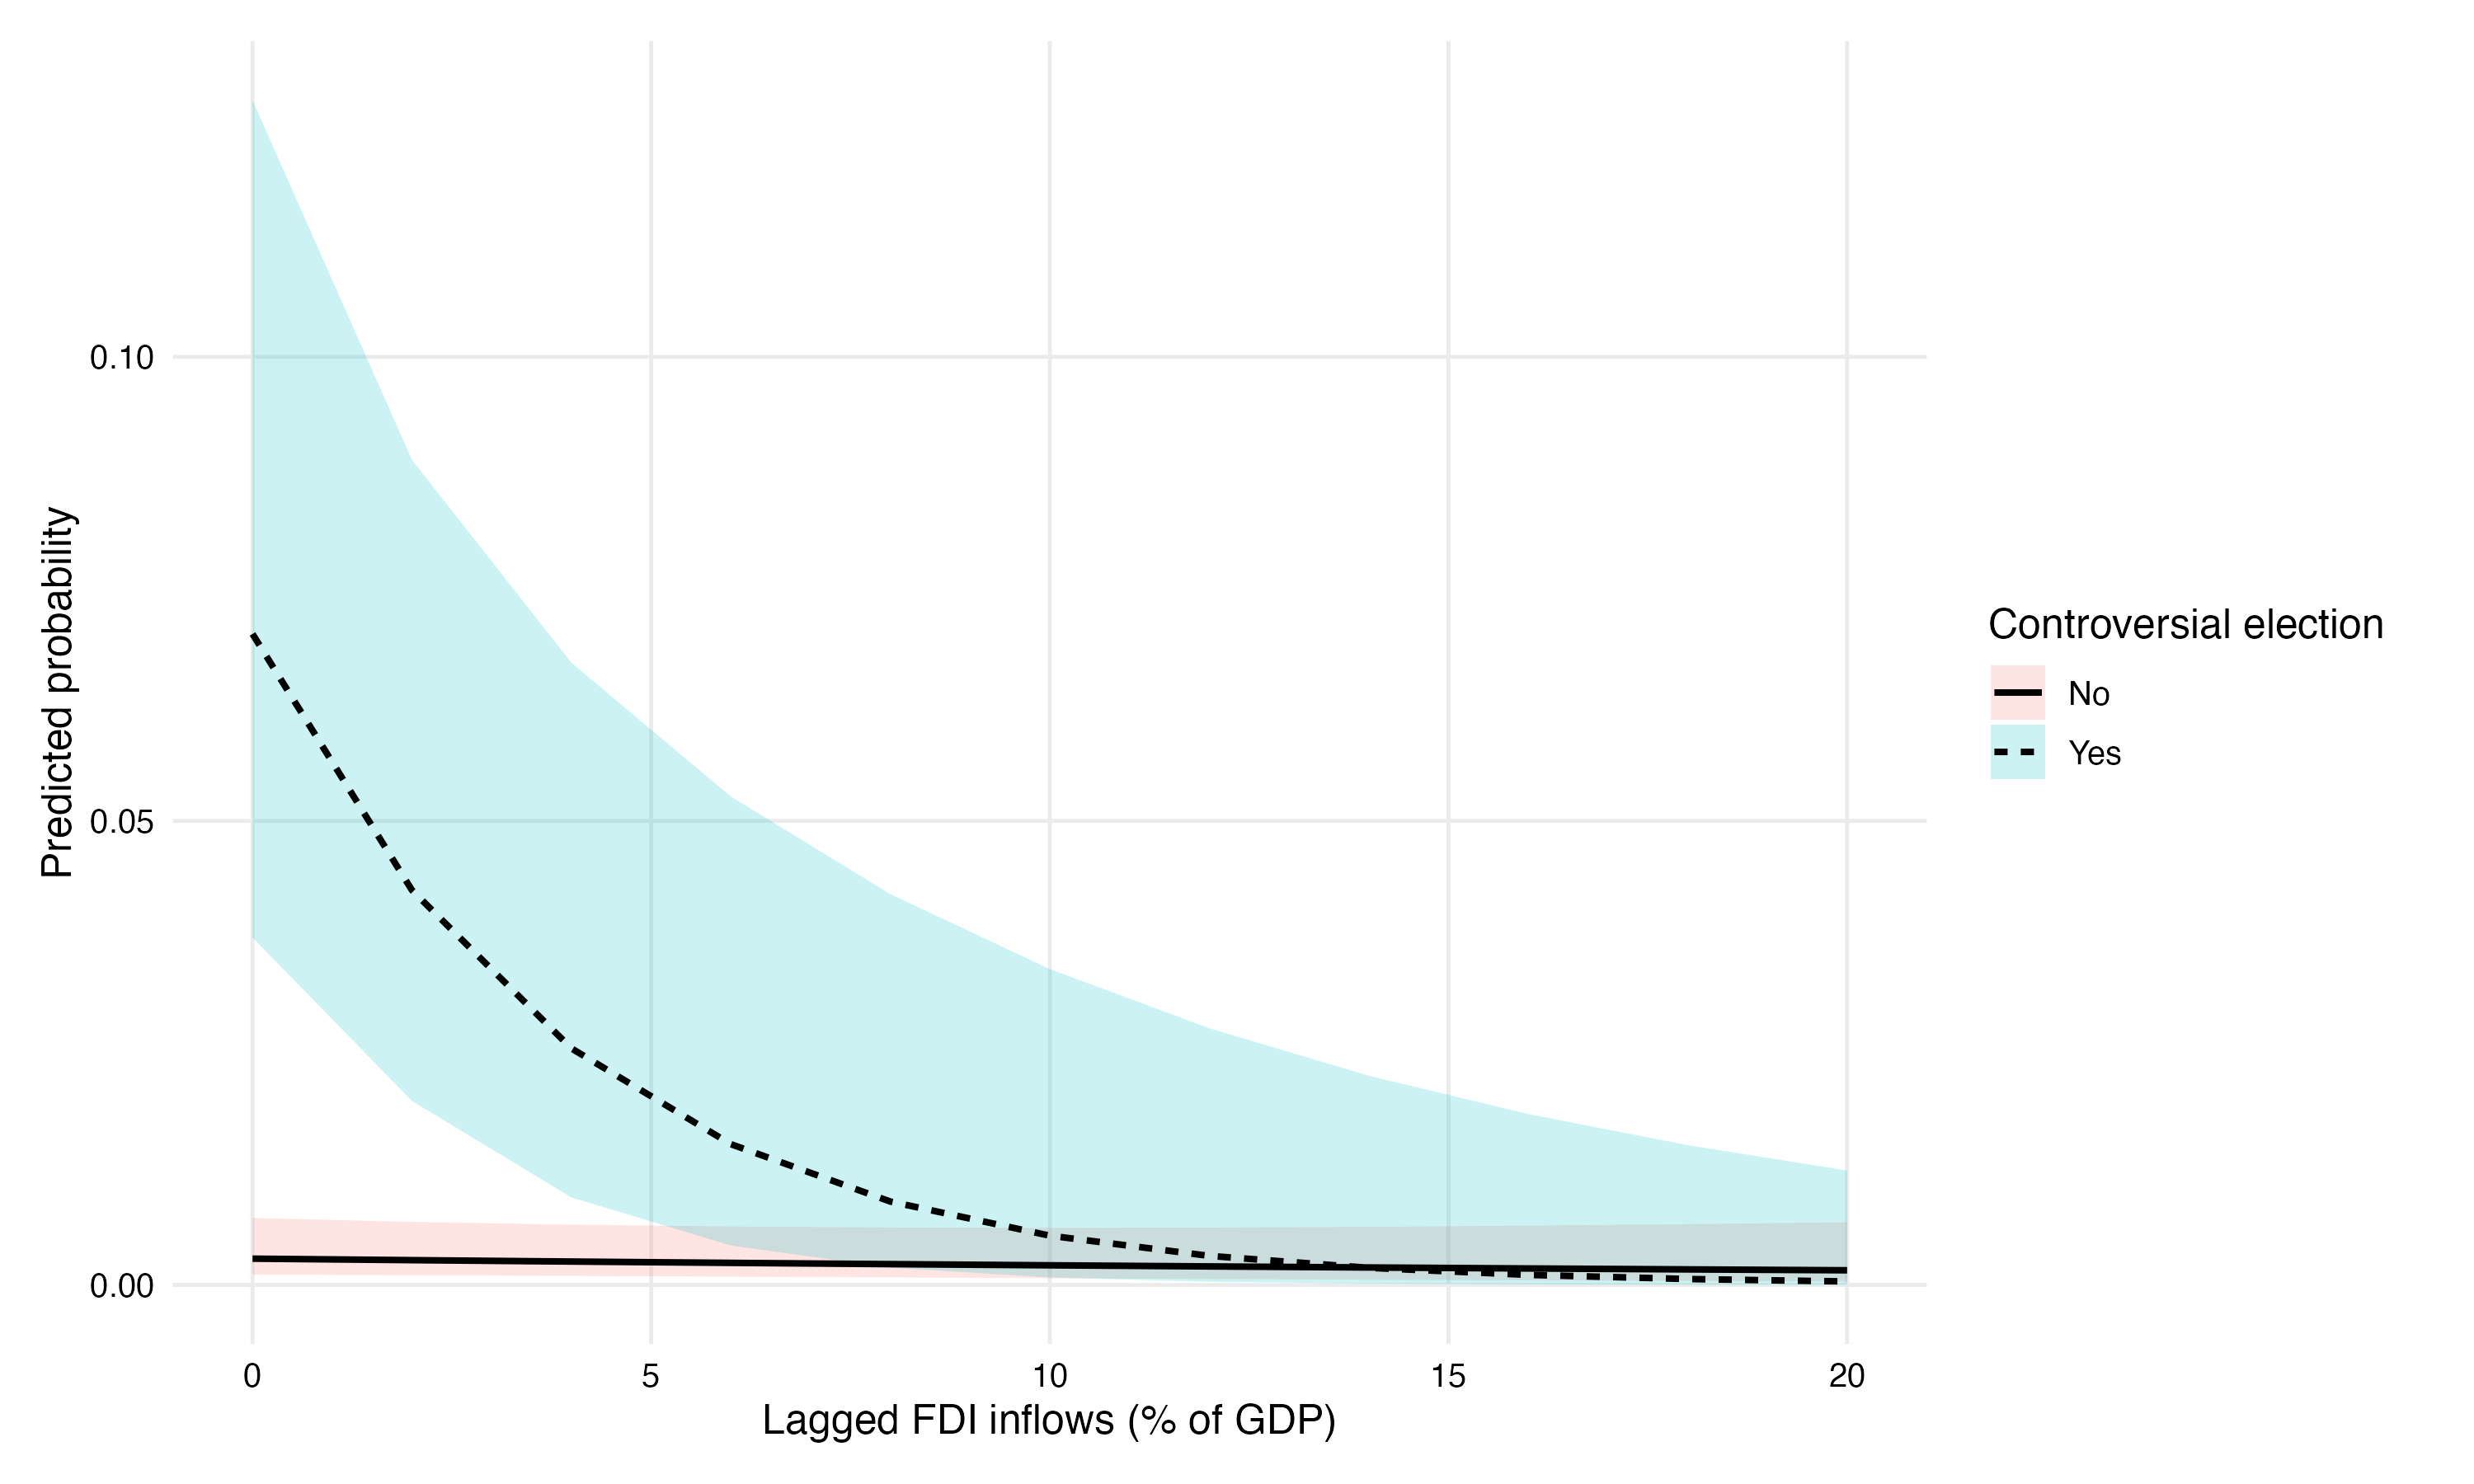
\includegraphics[width=0.86\textwidth]{figures/figure_2_fdi_by_election_status.png}
		\caption{Replication of the article's Figure 2: predicted probability of democratic sanctions by lagged FDI inflows and controversial election status.}
		\label{fig:replicated_figure2}
	\end{figure}
	
	The replicated figure tracks the original article's interpretation closely. When controversial elections occur, the predicted probability of democratic sanctions declines as FDI rises. In other words, economically costly targets appear more protected precisely in the setting where the trigger is normatively meaningful but less overwhelming than a coup. This is an important part of the original paper's contribution, because it shows that selectivity is not limited to static sender-target relationships. It is also visible in how senders react to weaker trigger events.
	
	Taken together, the main replication reproduces the paper's core empirical claims well. The strongest evidence concerns the central trigger findings and the selective-targeting patterns around political closeness and FDI. That is enough to support the original paper's main argument in a course replication setting.
	
	\FloatBarrier
	
	\section{Replication Extension}
	
	%\subsection*{Motivation}
	
	My extension asks whether the original paper's weaker-trigger logic also operates through geopolitical alignment, not only through economic exposure. This idea follows directly from the paper's own theory. Von Soest and Wahman argue that Western democratic sanctions are selective and that this selectivity should be especially visible for weaker triggers like controversial elections, because those cases leave senders more discretion than coups. They already demonstrate that logic once through the controversial election $\times$ FDI interaction in Model 7 and Figure 2. At the same time, one of their strongest substantive findings in the selective-targeting models is that politically closer regimes are less likely to be sanctioned at all. That naturally suggests a further question: if weaker triggers permit more strategic selectivity, might highly aligned regimes be especially protected from sanctions after controversial elections?

	
	\subsection*{Operationalization and modelling choice}
	
	The extension is implemented in Section 8 of the final replication script. I first build one common estimation sample, then define a new dummy variable, \texttt{high\_polclose}, equal to 1 for the top quartile of \texttt{lagree2un\_westimp2} in that estimation sample and 0 otherwise. I then estimate two models on the exact same sample: a baseline model without the interaction and an interaction model with controversial election $\times$ high political closeness.
	
	I chose this threshold specification for both theoretical and empirical reasons. Theoretically, the argument is not simply that every marginal increase in political closeness should linearly reduce sanctioning after controversial elections. The paper's logic is more consistent with a protection story: weaker triggers give senders room to shield especially friendly or strategically aligned regimes. A top-quartile indicator captures that idea more directly than a smooth linear interaction.
	
	Empirically, the continuous interaction did not behave well enough to justify being the final extension. In earlier exploratory versions, the controversial election $\times$ political closeness interaction was negative in sign but highly imprecise, with interaction estimates of $-1.956$ (SE $3.229$) and $-2.184$ (SE $3.912$). That made it difficult to defend a clean linear moderation story. The threshold formulation is therefore not a post hoc fishing exercise so much as a more interpretable and more theory-consistent way of testing whether especially aligned regimes appear somewhat protected in weaker-trigger scenarios.
	
	The key code block for this extension is shown below.
	
	\lstinputlisting[
	language=R,
	firstline=646,
	lastline=681,
	caption={Core extension code: common estimation sample and high-political-closeness threshold.}
	]{/Users/jakoblutkemeier/Documents/projects/replication-project-democratic-sanctions/code/replication_analysis.R}
	
	\subsection*{Extension results}
	
	\begin{table}
	\centering
	\begin{talltblr}[         %% tabularray outer open
		caption={Replication extension: political closeness threshold interaction},
		]                     %% tabularray outer close
		{                     %% tabularray inner open
			colspec={Q[]Q[]Q[]},
			hline{2}={1-3}{solid, black, 0.05em},
			hline{26}={1-3}{solid, black, 0.05em},
			hline{1}={1-3}{solid, black, 0.08em},
			hline{27}={1-3}{solid, black, 0.08em},
			column{2-3}={}{halign=c},
			column{1}={}{halign=l},
		}                     %% tabularray inner close
		&  \shortstack{Baseline\\(HTW Western)} & \shortstack{Interaction\\(HTW Western)} \\
		Coup & \num{5.119}*** & \num{5.074}*** \\
		& (\num{0.863}) & (\num{0.849}) \\
		Controversial election & \num{2.817}*** & \num{3.123}*** \\
		& (\num{0.467}) & (\num{0.508}) \\
		High political closeness (top quartile) & \num{-1.295}+ & \num{-0.590} \\
		& (\num{0.775}) & (\num{0.816}) \\
		Protests & \num{0.109}* & \num{0.110}* \\
		& (\num{0.053}) & (\num{0.055}) \\
		GDP per capita growth ($t-1$) & \num{-0.012} & \num{-0.017} \\
		& (\num{0.022}) & (\num{0.023}) \\
		Inflation ($t-1$) & \num{0.029}** & \num{0.026}* \\
		& (\num{0.011}) & (\num{0.011}) \\
		GDP per capita (\$1,000s, $t-1$) & \num{-0.158}* & \num{-0.151}* \\
		& (\num{0.070}) & (\num{0.067}) \\
		Non-democratic sanction ($t-1$) & \num{0.624} & \num{0.734} \\
		& (\num{0.616}) & (\num{0.609}) \\
		Time since last sanction & \num{-1.628}* & \num{-1.642}* \\
		& (\num{0.651}) & (\num{0.648}) \\
		Time since last sanction$^2$ & \num{0.208}* & \num{0.208}* \\
		& (\num{0.097}) & (\num{0.097}) \\
		Time since last sanction$^3$ & \num{-0.008}+ & \num{-0.008}+ \\
		& (\num{0.004}) & (\num{0.004}) \\
		Controversial election $\times$ high political closeness &  & \num{-1.784} \\
		&  & (\num{1.257}) \\
		N & \num{1388} & \num{1388} \\
	\end{talltblr}
\end{table}
	
	The main extension table (Table 4) suggests a pattern that is theoretically interesting but inferentially uncertain. The interaction points in the expected negative direction: after controversial elections, regimes in the highest political-closeness category appear less likely to face democratic sanctions than less aligned regimes. This is consistent with the paper's broader sender-cost logic and with the idea that weaker triggers leave more room for strategic discretion. However, the evidence is not strong enough to support a decisive claim. The interaction is better viewed as suggestive evidence than as a firm new result.
	
	That cautious interpretation becomes clearer when the model table is paired with a simple descriptive summary.
	
	\begin{table}
\centering
\begin{talltblr}[         %% tabularray outer open
caption={Observed sanction rates by election status and political closeness},
]                     %% tabularray outer close
{                     %% tabularray inner open
colspec={Q[]Q[]Q[]Q[]Q[]},
hline{2}={1-5}{solid, black, 0.05em},
hline{1}={1-5}{solid, black, 0.08em},
hline{6}={1-5}{solid, black, 0.08em},
column{1-5}={}{halign=l},
}                     %% tabularray inner close
election\_status & political\_closeness & N & Sanctions & Sanction rate \\
Controversial election & Lower 3 quartiles & \num{59.000} & \num{10.000} & \num{0.169} \\
Controversial election & Top quartile & \num{44.000} & \num{1.000} & \num{0.023} \\
No controversial election & Lower 3 quartiles & \num{982.000} & \num{23.000} & \num{0.023} \\
No controversial election & Top quartile & \num{303.000} & \num{3.000} & \num{0.010} \\
\end{talltblr}
\end{table}

	
	The descriptive support table (Table 5) is useful because it shows the underlying pattern more directly than the interaction coefficient alone. The key comparison is the sanction rate after controversial elections in the top political-closeness quartile versus the lower three quartiles. In substantive terms, the descriptive evidence points in the same direction as the model: highly aligned regimes appear somewhat less exposed to sanctions after controversial elections. At the same time, this support is descriptive rather than dispositive. It does not eliminate uncertainty about model dependence, sample size, or the sharpness of the threshold.
	
	I also conducted a robustness check to assess whether this pattern depended too heavily on one specific operationalisation. First, I varied the threshold used to define \texttt{high\_polclose}. The interaction remained negative under nearby one-year threshold choices, which suggests that the substantive pattern is not entirely driven by the top-quartile cutoff alone. Second, I tested lag sensitivity by re-estimating the extension with a two-year lag of political closeness rather than the one-year lag used in the main specification. In that version, the interaction weakened and no longer pointed consistently in the same direction. Taken together, these robustness checks suggest that the extension is plausible, but also specification-sensitive and therefore not decisive.
	
	For that reason, I do not treat the extension as overturning or fundamentally revising the original article. Rather, it modestly extends the paper's logic. If controversial elections are weaker triggers that permit more strategic selectivity, that selectivity may operate through geopolitical alignment as well as through economic exposure. The extension is therefore useful mainly as a theory-consistent probe, not as a new definitive mechanism.
	\FloatBarrier
	
	\section{Discussion and Conclusion}
	
	The replication was substantively successful for the paper's core results. The main patterns around coups, controversial elections, selective targeting, and the FDI/election relationship were recovered closely enough to support the central argument of the original study. Most importantly, the replication reproduces the paper's central claim that democratic sanctions are not simply imposed on the most autocratic regimes. They are more likely after dramatic trigger events and are shaped by strategic considerations about vulnerability and sender costs.
	
	The extension adds a plausible test of whether the paper's ``weaker triggers permit more strategic selectivity'' logic also applies to geopolitical alignment, operationalized as controversial election $\times$ high political closeness. It does not overturn the paper, establish a new decisive mechanism, or provide strong causal evidence. It is better understood as a modest, theory-consistent probe of whether highly aligned regimes may be somewhat protected from sanctions after controversial elections.
	
	The limitations are therefore asymmetrical. The replication is strong for the core findings, but the extension is much more sample- and specification-sensitive. The interaction evidence is imprecise, model-fit gains are marginal, and the descriptive pattern is more convincing than the formal inference. For that reason, the extension should be interpreted cautiously rather than presented as a firm result.
	
	Overall, this was a successful replication assignment. The main findings of \citet{vonsoestNotAllDictators2015} were reproduced credibly, and the project was extended with a modest, theoretically grounded additional analysis that is plausible, relevant, and appropriately cautious in its conclusions.


\bibliographystyle{apalike} 
\bibliography{replication_project} 
	
\end{document}